%%%%%%%%%%%%%%%%%%%%%%%%%%%%%%%%%%%%%%%%%
%
% CMPT 435
% Lab Zero
%
%%%%%%%%%%%%%%%%%%%%%%%%%%%%%%%%%%%%%%%%%

%%%%%%%%%%%%%%%%%%%%%%%%%%%%%%%%%%%%%%%%%
% Short Sectioned Assignment
% LaTeX Template
% Version 1.0 (5/5/12)
%
% This template has been downloaded from: http://www.LaTeXTemplates.com
% Original author: % Frits Wenneker (http://www.howtotex.com)
% License: CC BY-NC-SA 3.0 (http://creativecommons.org/licenses/by-nc-sa/3.0/)
% Modified by Alan G. Labouseur  - alan@labouseur.com, and Ryan Munger - ryan.munger1@marist.edu
%
%%%%%%%%%%%%%%%%%%%%%%%%%%%%%%%%%%%%%%%%%

%----------------------------------------------------------------------------------------
%	PACKAGES AND OTHER DOCUMENT CONFIGURATIONS
%----------------------------------------------------------------------------------------

\documentclass[letterpaper, 10pt]{article} 

\usepackage[english]{babel} % English language/hyphenation
\usepackage{graphicx}
\usepackage[lined,linesnumbered,commentsnumbered]{algorithm2e}
\usepackage{listings}
\usepackage{fancyhdr} % Custom headers and footers
\pagestyle{fancyplain} % Makes all pages in the document conform to the custom headers and footers
\usepackage{lastpage}
\usepackage{url}
\usepackage{xcolor}
\usepackage{titlesec}

% Stolen from https://www.overleaf.com/learn/latex/Code_listing 
\definecolor{codegreen}{rgb}{0,0.6,0}
\definecolor{codegray}{rgb}{0.5,0.5,0.5}
\definecolor{codepurple}{rgb}{0.58,0,0.82}
\definecolor{backcolour}{rgb}{0.95,0.95,0.92}

\lstdefinestyle{mystyle}{
    backgroundcolor=\color{backcolour},   
    commentstyle=\color{codegreen},
    keywordstyle=\color{magenta},
    numberstyle=\tiny\color{codegray},
    stringstyle=\color{codepurple},
    basicstyle=\ttfamily\footnotesize,
    breakatwhitespace=false,         
    breaklines=true,                 
    captionpos=b,                    
    keepspaces=true,                 
    numbers=left,                    
    numbersep=5pt,                  
    showspaces=false,                
    showstringspaces=false,
    showtabs=false,                  
    tabsize=2
}
\lstset{style=mystyle, language=c++}


\fancyhead{} % No page header - if you want one, create it in the same way as the footers below
\fancyfoot[L]{} % Empty left footer
\fancyfoot[C]{page \thepage\ of \pageref{LastPage}} % Page numbering for center footer
\fancyfoot[R]{}

\renewcommand{\headrulewidth}{0pt} % Remove header underlines
\renewcommand{\footrulewidth}{0pt} % Remove footer underlines
\setlength{\headheight}{13.6pt} % Customize the height of the header

%----------------------------------------------------------------------------------------
%	TITLE SECTION
%----------------------------------------------------------------------------------------

\newcommand{\horrule}[1]{\rule{\linewidth}{#1}} % Create horizontal rule command with 1 argument of height

\title{	
   \normalfont \normalsize 
   \textsc{CMPT 435 - Fall 2024 - Dr. Labouseur} \\[10pt] % Header stuff.
   \horrule{0.5pt} \\[0.25cm] 	% Top horizontal rule
   \huge Assignment One -- Structures \& Sorting\\     	    % Assignment title
   \horrule{0.5pt} \\[0.25cm] 	% Bottom horizontal rule
}

\author{Ryan Munger \\ \normalsize Ryan.Munger1@marist.edu}

\date{\normalsize\today} 	% Today's date.

\begin{document}

\maketitle % Print the title

%----------------------------------------------------------------------------------------
%   CONTENT SECTION
%----------------------------------------------------------------------------------------

% - -- -  - -- -  - -- -  -
\section{Introduction}
\subsection{Goals}
Assignment 1 instructed us to create the elementary data structures \textit{Stack} and \textit{Queue} using a node implementation. We then checked a list of items for palindromes using these data structures and also sorted the list using selection, insertion, merge, and quick sorts.
\subsection{Write-up Format}
    In this report I will describe the logic being presented. Below the text explanation, relevant code will follow. I implemented the foundational parts of this assignment in both C++ and Ada. I was originally planning to use Pascal, but became frustrated with the nuances of different versions and compilers. As I was writing Pascal, I found it incredibly similar to a language I have seen before - Ada (Not like its based on Pascal or anything...). Before you ask, I work in the defense industry. I used this as an opportunity to actually learn Ada so that I can be better at my job with Lockheed Martin. I used Alire to build and run my Ada code. Alire is extremely similar to Cargo for Rust. Under the hood, it uses GNAT to build the Ada program. Long story short, walrus assignment is pretty cool. I will attempt to sprinkle in some jokes for you!
\subsection{Limerick of Luck}
Limerick of Luck would make a good magic item... \\
I suggest adding Nogard Dragon as a new palindrome! \\
\noindent
All programmers revere the power of sorting \\
Especially after conducting it with no importing. \\
    \hspace*{1.5em}Despite some having large big-oh, \\
    \hspace*{1.5em}Merge sort hasn't yet delivered a deathblow, \\
Allowing us to experiment with algorithms so cavorting. \\
\section{Nodes, Linked Lists, Stacks, \& Queues}
\subsection{Making a Node}
Nodes are the foundations of linked lists. Other data structures including stacks and queues are special forms of linked lists. To create nodes capable of forming a singly linked list (meaning nodes know where to find the next node but not the previous), they need a value and a pointer to the following node. I used a template in my implementation so that we can use the nodes with any type of data. A nodes value and next node can be accessed publicly. The Ada implementation is limited to char nodes.
\lstinputlisting[linerange={8-12}, firstnumber=8]{assignment1.cpp}
\lstinputlisting[language=Ada, linerange={10-17}, firstnumber=10]{assignment1.adb}
\subsection{Testing our Nodes}
Code:

\lstinputlisting[linerange={332-344}, firstnumber=332]{assignment1.cpp}
Output:
\lstinputlisting[linerange={1-4}, firstnumber=1]{output.txt}
Code:
\lstinputlisting[language=Ada, linerange={137-149}, firstnumber=137]{assignment1.adb}
Output:
\lstinputlisting[linerange={3-6}, firstnumber=3]{ada_output.txt}
\subsection{Stacks \& Queues}
Nodes can link together to form linked lists. Stacks and queues are linked lists with special rules. Stacks can only be managed from the top, similar to a stack of dining hall plates. You can add or remove from the top of the stack but nothing more (this is called LIFO - Last In First Out). Queues are like a line to enter a dining hall; you can only add things to the end of the line and take from the front (FIFO - First In First Out).
\newline
A stack needs - push (add to stack), pop (remove), isEmpty (see if it has anything in it), and optionally, size \& peek. Queues need - enqueue (add to end of line), dequeue (remove from front), isEmpty, and optionally, size \& peek. All of these operations are in constant time (as my queue has a tail pointer). \\
\newline
The stack needs a pointer to the top of the stack just as a queue keeps track of its head and tail.\\
\newpage
\textbf{Stack Declaration:}
\lstinputlisting[linerange={14-31}, firstnumber=14]{assignment1.cpp}
\lstinputlisting[language=Ada, linerange={20-23}, firstnumber=20]{assignment1.adb}
\textbf{Stack Push:}
\begin{enumerate}
    \item Store new data into a node.
    \item The new next node is the current top.
    \item The new top is the new node.
    \item Increase stack size (optional).
\end{enumerate}
\lstinputlisting[linerange={37-44}, firstnumber=37]{assignment1.cpp}
\lstinputlisting[language=Ada, linerange={33-39}, firstnumber=33]{assignment1.adb}
\newpage
\textbf{Stack Pop:}
\begin{enumerate}
    \item Ensure stack not empty.
    \item Note the value of current top.
    \item Make the node after the current top the new top.
    \item Reduce stack size (optional).
    \item Delete the old node from memory (garbage collection).
    \item Return the value of the old top node.
\end{enumerate}
\lstinputlisting[linerange={46-58}, firstnumber=46]{assignment1.cpp}
\lstinputlisting[language=Ada, linerange={42-54}, firstnumber=42]{assignment1.adb}
\textbf{Stack isEmpty:}
\begin{enumerate}
    \item Returns true if the top of the stack is a nullptr.
\end{enumerate}
\textbf{Stack getSize:}
\begin{enumerate}
    \item Returns value of size attribute.
\end{enumerate}
\textbf{Stack Peek:}
\begin{enumerate}
    \item Returns the value of the top node without popping it.
\end{enumerate}
\hrule
\vspace{.25cm}
Why did the stack go to therapy? - \textit{It keeps pushing things down...}\\
\hrule
\vspace{.25cm}
\textbf{Testing Stack: } \\
Code:
\lstinputlisting[linerange={349-357}, firstnumber=349]{assignment1.cpp}
Output:
\lstinputlisting[linerange={6-9}, firstnumber=6]{output.txt}
\noindent
As previously mentioned, the queue class will need to have a pointer to the first and the last node to work in constant time. It is possible traverse the queue to obtain the final node, but the trade off between memory and time is worth it in this case to store an additional pointer. \\
\textbf{Queue Implementation:}
\lstinputlisting[linerange={70-88}, firstnumber=70]{assignment1.cpp}
\lstinputlisting[language=Ada, linerange={26-30}, firstnumber=26]{assignment1.adb}
\newpage
\textbf{Queue Enqueue:}
\begin{enumerate}
    \item Create a new node with the new value.
    \item If queue empty, new node is the head.
    \item Otherwise, set the current tail's next value to the new node.
    \item Make the new node the tail.
    \item Increment size (optional).
\end{enumerate}
\lstinputlisting[linerange={94-108}, firstnumber=94]{assignment1.cpp}
\lstinputlisting[language=Ada, linerange={56-71}, firstnumber=56]{assignment1.adb}

\textbf{Queue Dequeue:}
\begin{enumerate}
    \item Make sure queue is not empty.
    \item Note the value of the current head.
    \item Set the new head to the current head's next.
    \item Free up memory from the now old head.
    \item Check if the head is now null, if so, set tail to null.
    \item Decrement size (optional). 
    \item Return the value of now the old head node.
\end{enumerate}
\lstinputlisting[linerange={110-125}, firstnumber=110]{assignment1.cpp}
\lstinputlisting[language=Ada, linerange={73-91}, firstnumber=73]{assignment1.adb}
\textbf{Queue isEmpty:}
\begin{enumerate}
    \item Return true if the head and the tail are null.
\end{enumerate}
\textbf{Queue peekFront:}
\begin{enumerate}
    \item Return value of head node.
\end{enumerate}
\textbf{Queue peekBack:}
\begin{enumerate}
    \item Return value of tail node.
\end{enumerate}
\textbf{Queue getSize:}
\begin{enumerate}
    \item Return value of size attribute.
\end{enumerate}

\hrule
\vspace{.25cm}
Why did the stack break up with the queue? - \textit{It found a priority queue to put it first...}\\
\hrule
\vspace{.25cm}
\textbf{Testing Queue: } \\ 
Code:
\lstinputlisting[linerange={359-367}, firstnumber=359]{assignment1.cpp}
Output:
\lstinputlisting[linerange={11-14}, firstnumber=11]{output.txt}

\subsection{Palindrome Checking: A Stack \& Queue Use Case}
A palindrome is word/phrase that reads the same forward and backwards. For our implementation, we will ignore spaces and case. "Racecar" is a palindrome because the letters read the same front to back and back to front. "Nogard Dragon" should be in the ones we are checking because I think its cool (is that not reason enough?). We read in the list of words/phrases to check from magicitems.txt and determine if it is a palindrome by: \\
\begin{enumerate}
    \item Declaring a stack and a queue.
    \item For each char in the item, push/enqueue each char to each respective data structure in lower case if it is not a space.
    \item Pop each element from the stack and dequeue each element from the queue. If they do not match, it is not a palindrome! (As stack has the word in reverse order).
\end{enumerate}

\textbf{Read in magic items:}
\lstinputlisting[linerange={148-160}, firstnumber=148]{assignment1.cpp}
\lstinputlisting[language=Ada, linerange={120-135}, firstnumber=120]{assignment1.adb}

\textbf{Check for palindromes:}
\lstinputlisting[linerange={162-181}, firstnumber=162]{assignment1.cpp}
\lstinputlisting[language=Ada, linerange={93-117}, firstnumber=93]{assignment1.adb}
\textbf{Results:}
% just chose a lang that doesnt have keywords in the output %
\lstinputlisting[language=Ant, linerange={8-22}, firstnumber=8]{ada_output.txt}
\hrule
\vspace{.25cm}
Why is 'palindrome' not a palindrome? Dr. Labouseur and other detail oriented people surely don't get annoyed by this...\\
\hrule

\section{Sorting}
\subsection{Introduction}
In this section we will sort our list alphabetically from least (a) to greatest (z). The $\leq$ 
 relation is a \textbf{total order} and must uphold the following: \\
\begin{enumerate}
    \item Reflexivity: For all x in S, $x \leq x$.
    \item Antisymmetry: For all x, y in S, if $x \leq y$ and $y \leq x$, then $x = y$.
    \item Transitivity: For all x, y, z in S, if $x \leq y$ and $y \leq z$, then $x \leq z$.
\end{enumerate}
\smaller Good 'ol discrete math... \\
\normalsize
I implemented this section in c++ only.
\subsection{Unsorting?}
A truly unsorted array is one in which the elements are randomly positioned. This array can technically be sorted (the basis for the monkey/bogo sort), but we won't actually know until we check. Since we are implementing several sorting algorithms, we will need to unsort/shuffle the array between sorts. A good algorithm to do this randomly \& in place is the Knuth/Fisher Yates Shuffle. It iterates through each data point in an array, picking a random index between current index and all remaining indices and swaps the values between the two.
\lstinputlisting[linerange={140-146}, firstnumber=140]{assignment1.cpp}
\subsection{Selection Sort}
Selection sort is an in place sort that organizes an array using a nested loop. Selection sort iterates through the array except for the portion is has already sorted and finds the minimum value (when doing $\leq$). Once we find the minimal element, we swap it with the current index. This way, if we are on array index 2 (starting at 0) we would swap in the 3rd smallest value. This algorithm works in $O(n^2)$ time because the outer loop runs $n$ times and the inner loop has to iterate over the entire array it hasn't yet sorted. Despite the fact that the inner loop decreases in iterations as the sort progresses, this is still quadratic time because the number of the inner iterations depends on the size of the input; therefore $n*n$ comparisons (where $n$ is size of the array). A more precise characterization of this algorithm is as follows: \\
Total comparisons: $(n - 1) + (n - 2) + \cdots + 1 = \sum_{i=1}^{n-1} i$ \\
$\sum_{i=1}^{n-1} i = \frac{(n-1)+1}{2}(n-1) = \frac{1}{2}n(n-1) = \frac{1}{2}(n^2-n)$ \\
As we can see, in this case $n^2$ dominates therefore the algorithm is $O(n^2)$. Using this formula on our array of 666 elements, we can expect $\frac{1}{2}(666^2-666)$ or 221,445 comparisons to be made. It will always take this exact number of comparisons, even if the array is presorted or totally unsorted. 
\lstinputlisting[linerange={192-209}, firstnumber=192]{assignment1.cpp}
\hrule
\vspace{.25cm}
Why did selection sort's girlfriend leave him? - \textit{Turns out checking out every option before selecting her wasn't flattering...}\\
\hrule
\subsection{Insertion Sort}
Insertion sort is an in place sort that is similar to selection sort. Instead of iterating through the entire array to find the item destined for the next position in the array, insertion sort simply grabs the next item and puts it in the correct location. Instead of searching forward for the most optimal value, insertion sort \textit{inserts} the next value it is looking at in its correct relative position. The exact time complexity of this algorithm is difficult to calculate directly as it depends on the order the array is in, but the worst case is that the inner loop will have to iterate through the entire sorted portion of the array to find the correct location for each item.
The worst case makes insertion sort $O(n^2)$ since the length of the inner array is approximately $n/2$ on average. A complexity of $n*\frac{1}{2}n$ without constants is $n^2$. For our array of 666 elements, we can expect between best case (sorted: $n-1$ comparisons) or worst case (same as selection sort), or 665 - 221,445. Averaging these, we should expect generally around 111,388 comparisons.
\lstinputlisting[linerange={212-231}, firstnumber=212]{assignment1.cpp}
\subsection{Merge Sort}
Merge sort is a divide and conquer algorithm that is not in place. It works by recursively dividing the array into smaller subarrays and sorting those subarrays. The subarrays are sorted by dividing them just as we did with the input array. The base case is an array of size one, which is sorted! Once we reach subarrays of size one, we then merge them back together all the way up the recursive tree until we have a completely sorted array.

To be concise, merge sort divides the array into halves, sorts each half, and then merges the sorted halves back together (and does so for each half of the half... etc.). This process is repeated until the entire array is sorted.
Dividing the array is a constant time operation. There are \(log_2n \) divides as the array is cut in half each recursion. Each divide step must also be merged back together. There are n items to merge back together at each subarray size. This operation will take $n$ time. Therefore, the time complexity is $O(nlog_2n)$. We should then expect $666*log_2666$ which is 6,244 comparisons.\\
\newline
Merge sort is driven by a recusrively called function that
\begin{enumerate}
    \item Checks if the subarray can be divided further. If not, array is of size 1 and is sorted (base case).
    \item Makes a recursive call to divide the subarray further if it can.
    \item Calls a helper function to stitch the two halves back together in a sorted order.
\end{enumerate}
\lstinputlisting[linerange={280-295}, firstnumber=280]{assignment1.cpp}
The helper function first builds the two subarrays we are to work with (the only subarrays that get to this function are sorted). We then write the subarray data back into the original array in the correct order. Combining the two arrays is simple as we can just use a while loop to see which next element in either array is smaller since the subarrays are sorted. Once this is completed, the two subarrays have been merged successfully.
\lstinputlisting[linerange={233-277}, firstnumber=233]{assignment1.cpp}
\hrule
\vspace{.25cm}
A mad scientest has created a self sorting array! He pulls back the curtain and to the crowd's dismay yells: \textit{"BEHOLD! A array of size one!!"}
\vspace{.25cm}
\hrule
\newpage
\subsection{Quick Sort}
Quick sort also utilizes a divide and conquer methodology. Similar to merge sort, it recursively divides the array using a pivot value. It partitions the array by splitting the array at the pivot value by grouping items less than the pivot into one partition and the rest into another. There are many different versions of the partition algorithm, but I chose the Lomuto partition as it is easy to understand. Lomuto partition keeps track of the indices of smaller elements and keep swapping, always using the last element as the pivot. The image below from GeeksforGeeks.org does a great job of visualizing the process. \\
\begin{figure}[h]
    \centering
    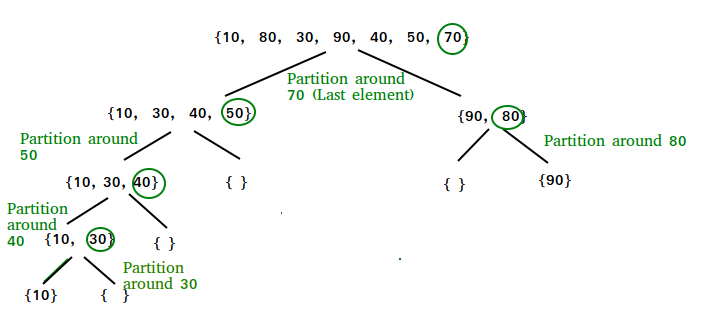
\includegraphics[width=1\linewidth]{quickSort.png}
    \caption{Lomuto Quick Sort}
    \label{fig:enter-label}
\end{figure}
\newline
The time complexity for quick sort is $O(nlog_2n)$ as there are rarely more than \(log_2n \) partitions (given we are choosing good pivots) and $n$ comparisons required for each partition to correctly order the elements around the pivot. The absolute worst case is that the pivot is always the largest or smallest element, which leaves us at $O(n^2)$, or 221,445 comparisons. On average however, we can expect $O(nlog_2n)$, or $666*log_2666$ which is 6,244 comparisons.\\
\newline
First, we have the recursive function: 
\begin{enumerate}
    \item Checks if the partition can be divided further. If not, array is of size 1 and is sorted (base case).
    \item Call a helper function to partition the array.
    \item Makes a recursive call to sort the partitions.
\end{enumerate}
\newpage
\lstinputlisting[linerange={320-328}, firstnumber=320]{assignment1.cpp} 
The helper function is a bit more complex (we are using Lomuto).
\begin{enumerate}
    \item Choose a pivot value (last element in partition).
    \item Locate the start index of the partition.
    \item Traverse partition and move all smaller elements to the left side of the pivot. This generally leaves the pivot toward the middle of the array. We can then again partition further.
\end{enumerate}
Once again, GeeksforGeeks.org has an excellent graphic: 
\begin{figure}[h]
    \centering
    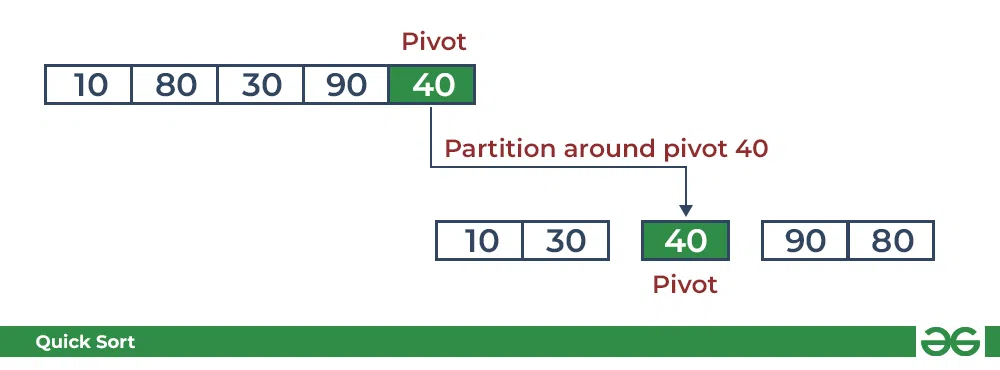
\includegraphics[width=1\linewidth]{pivoting.png}
    \caption{Pivoting}
    \label{fig:enter-label}
\end{figure}
\lstinputlisting[linerange={297-317}, firstnumber=296]{assignment1.cpp}
\hrule
\vspace{.25cm}
Why does quicksort have no friends? - \textit{It always pivots the conversation to talk about itself...}
\vspace{.25cm}
\hrule

\subsection{Comparing the Sorts}
In terms of time complexity, quick sort and merge sort easily pull ahead of selection and insertion. This does not mean that selection and insertion sorts are not useful. Selection sort is an excellent teaching exercise, is easy to understand, and employs minimal overhead \& swaps. Insertion sort is very quick to sort already sorted/near sorted arrays. Merge sort generally uses less comparisons than quick sort, but ends up with more overhead. Most in-built sorting libraries like sort() in Python use Timsort. Timsort is simply a hybrid sorting algorithm derived from ((merge sort or quick sort) and insertion sort). By using both algorithms, we can play on the strengths of each. By using merge sort to get the array almost sorted and insertion to finish the job, improvements are made. Since the code I implemented counts the comparisons for each sort, I will run it 20 times and average the results in a table below.

\begin{center}
\begin{tabular}{||c c c c||} 
 \hline
 Sort & Time Complexity & Expected & Actual\\ [0.5ex] 
 \hline\hline
 Selection Sort & \( O(n^2)\) & \(221,445\) & \(221,445\) \\
 \hline
 Insertion Sort & \( O(n^2)\) & \(111,388\) & \(112,609\) \\
 \hline
 Merge Sort & \( O(nlog_2n)\) & \(6,244\) & \(5,424\) \\
 \hline
 Quick Sort & \( O(nlog_2n)\) & \(6,244\) & \(6,760\) \\
 \hline
\end{tabular}
\\

\end{center}
Selection sort is exactly as expected since it always checks every element. Insertion sort did vary a bit, but is right on par with the expected. Merge sort performed well, as it is usually a bit faster than its Big-Oh. Quick sort lagged behind, but this is likely due to my suboptimal choice of the Lomuto partitioning algorithm.
\newpage
\section{Miscellaneous Lessons Learned}
If I learned anything, it is that the walrus operator is sick. I guess I learned a lot about Big Oh and sorting algorithms, but that pales in comparison. One thing I wished I knew is that you need to seed the random number generator in C++ or it will always give you the same numbers (seeding with current time is best). Aside from general Ada knowledge, I am satisfied with my newfound understanding of fundamental data structures and sorting algorithms. 
\newline
\hrule
\vspace{.25cm}
You really read this whole thing? \textbf{WOW!}
\vspace{.25cm}
\hrule
\end{document}